\label{sec:ionized_igm}

In this subsection, I describe the \lya\ emission from the ionized IGM. As mentioned
at the beginning of this section, I focus on \lya\ emission in the ionized IGM due to hydrogen recombinations.
As with \lya\ emitting galaxies, the ionized bubbles around galaxies also emits \lya\ photons through
recombinations of ionized hydrogen. The luminosity density of \lya\ emission in
some voxel of the simulation cubes can be defined using the following relationship,
\begin{equation}
  l_{\rm rec} = E_{\rm Ly\alpha} f_{\rm rec} \dot{n}_{\rm rec} \left( \textbf{x}, z \right),
\end{equation}
where $E_{\rm Ly\alpha}$ is the rest-frame energy of \lya\ photons, $f_{\rm rec}$ is the
fraction of recombinations that result in the emission of a \lya\ photon, and $\dot{n}_{\rm rec}$
is the comoving number density of recombinations occurring in the ionized IGM. The expression for the
number density of recombinations reads as,
\begin{equation}
  \dot{n}_{\rm rec} \left( \textbf{x}, z \right) = \alpha_{\rm A} n_{e} \left(z \right) n_{\textsc{HII}} \left(z \right),
\end{equation}
where $n_{e} = x_i \left( \textbf{x}, z \right) n_{b} \left( \textbf{x}, z \right)$,
$n_{\textsc{HII}} = n_{e} \left(4 - 4 Y_{\rm He} \right) /  \left(4 - 3 Y_{\rm He} \right)$ and $\alpha_{\rm A}$
is the comoving recombination coefficient. The comoving baryonic number density can be expressed using the
relationship below,
\begin{equation}
  n_{b} \left( \textbf{x}, z \right) = \bar{n}_{b, 0} \left( 1 + z\right)^3 \left[1 + \delta_{\rm nl} \left( \textbf{x}, z\right) \right],
\end{equation}
where $n_{b}$ is dependent on the non-linear density contrast, $\delta_{\rm nl} \left( \textbf{x}, z\right)$, and the
present-day mean baryonic number density, $\bar{n}_{b, 0} = 1.905 \times 10^{-7} \ \rm{cm}^{-3}$. Finally, the
comoving recombination coefficient, $\alpha_{\rm A}$, is defined below,
\begin{equation}
  \alpha_{\rm A} \approx 4.2 \times 10^{-13} \left( T_{\rm K} / 10^4 {\rm K} \right)^{-0.7} \left( 1 + z\right)^3 \ \left[\rm  cm^3 \ s^{-1} \right].
\end{equation}

The comoving number density of recombinations, $\dot{n}_{\rm rec}$, per pixel is simulated
by using \fastsim\ to evolve the kinetic gas temperature $T_k \left( \textbf{x}, z \right)$,
comoving baryonic number density $n_{b} \left( \textbf{x}, z \right)$, and the ionization
fraction $x_{i} \left( \textbf{x}, z \right)$ for each voxel in the simulation cube.
With the number density of recombinations calculated in each voxel, the luminosity
density of \lya\ emission in the ionized IGM can be calculated and converted to
a surface brightness using the following relationship,
\begin{equation}
I_{\nu}^{\rm rec} = y \left(z \right) d_A^2 \left(z \right) \frac{l_{\rm rec} \left( \textbf{x}, z \right)}{4 \pi d_L^2 \left( z \right)}.
\end{equation}

In reality, \lya\ emission from the ionized IGM also includes the scattered IGM \lya\
background whose main contributors are X-ray and UV heating, as well as the scattering of Lyman-n
photons emitted from galaxies by residual neutral hydrogen in the ionized IGM (\cite{2007MNRAS.376.1680P}).
For this work, I chose to neglect the contribution from this \lya\ background as its contribution
is subdominant to hydrogen recombination in the ionized IGM (roughly half the mean surface brightness)
and the galactic \lya\ contribution (about an order of magnitude lower) as found in \cite{2013ApJ...763..132S} and
\cite{2017ApJ...848...52H}. Adding in
the \lya\ background contribution in the future should be
trivial as \fastsim\ keeps track of this its emission when evolving the kinetic
gas temperature and the ionization field. The surface brightness
of \lya\ emission due to this background, $J_{\alpha} \left( \textbf{x}, z\right)$, can then be
calculated using the following expression (\cite{2013ApJ...763..132S}):

\begin{equation}
  I_{\nu} = \frac{6 E_{\text{Ly}\alpha}\, d_\textsc{a}^2 \left(z \right)}{\left( 1 + z\right)^2 d_\textsc{l}^2 \left( z \right)}\, J_{\alpha} \left( \textbf{x}, z \right).
\end{equation}

With all of the components of \lya\ emission during the EoR simulated and converted to surface brightnesses,
I then calculate the fluctuation field of \lya\ emission by summing over the individual
contributions to \lya\ emission from galaxies and the ionized IGM.
\begin{equation}
  \delta I_{\nu} \left(\textbf{x}, z \right) = \sum_i \frac{\nu I_{\nu, i} \left(\textbf{x}, z \right)}{\nu \bar{I}_{\nu} \left(z \right)} - 1
\end{equation}
This expression will to used to calculate the \lya\ auto-power spectrum and the 21\,cm-\lya\
cross-power spectrum in the following section. The slices through the simulated 21\,cm and the various
components of \lya\ emission cubes are shown in Figure \ref{fig:sims}.

\begin{figure}[p]
	\centering
	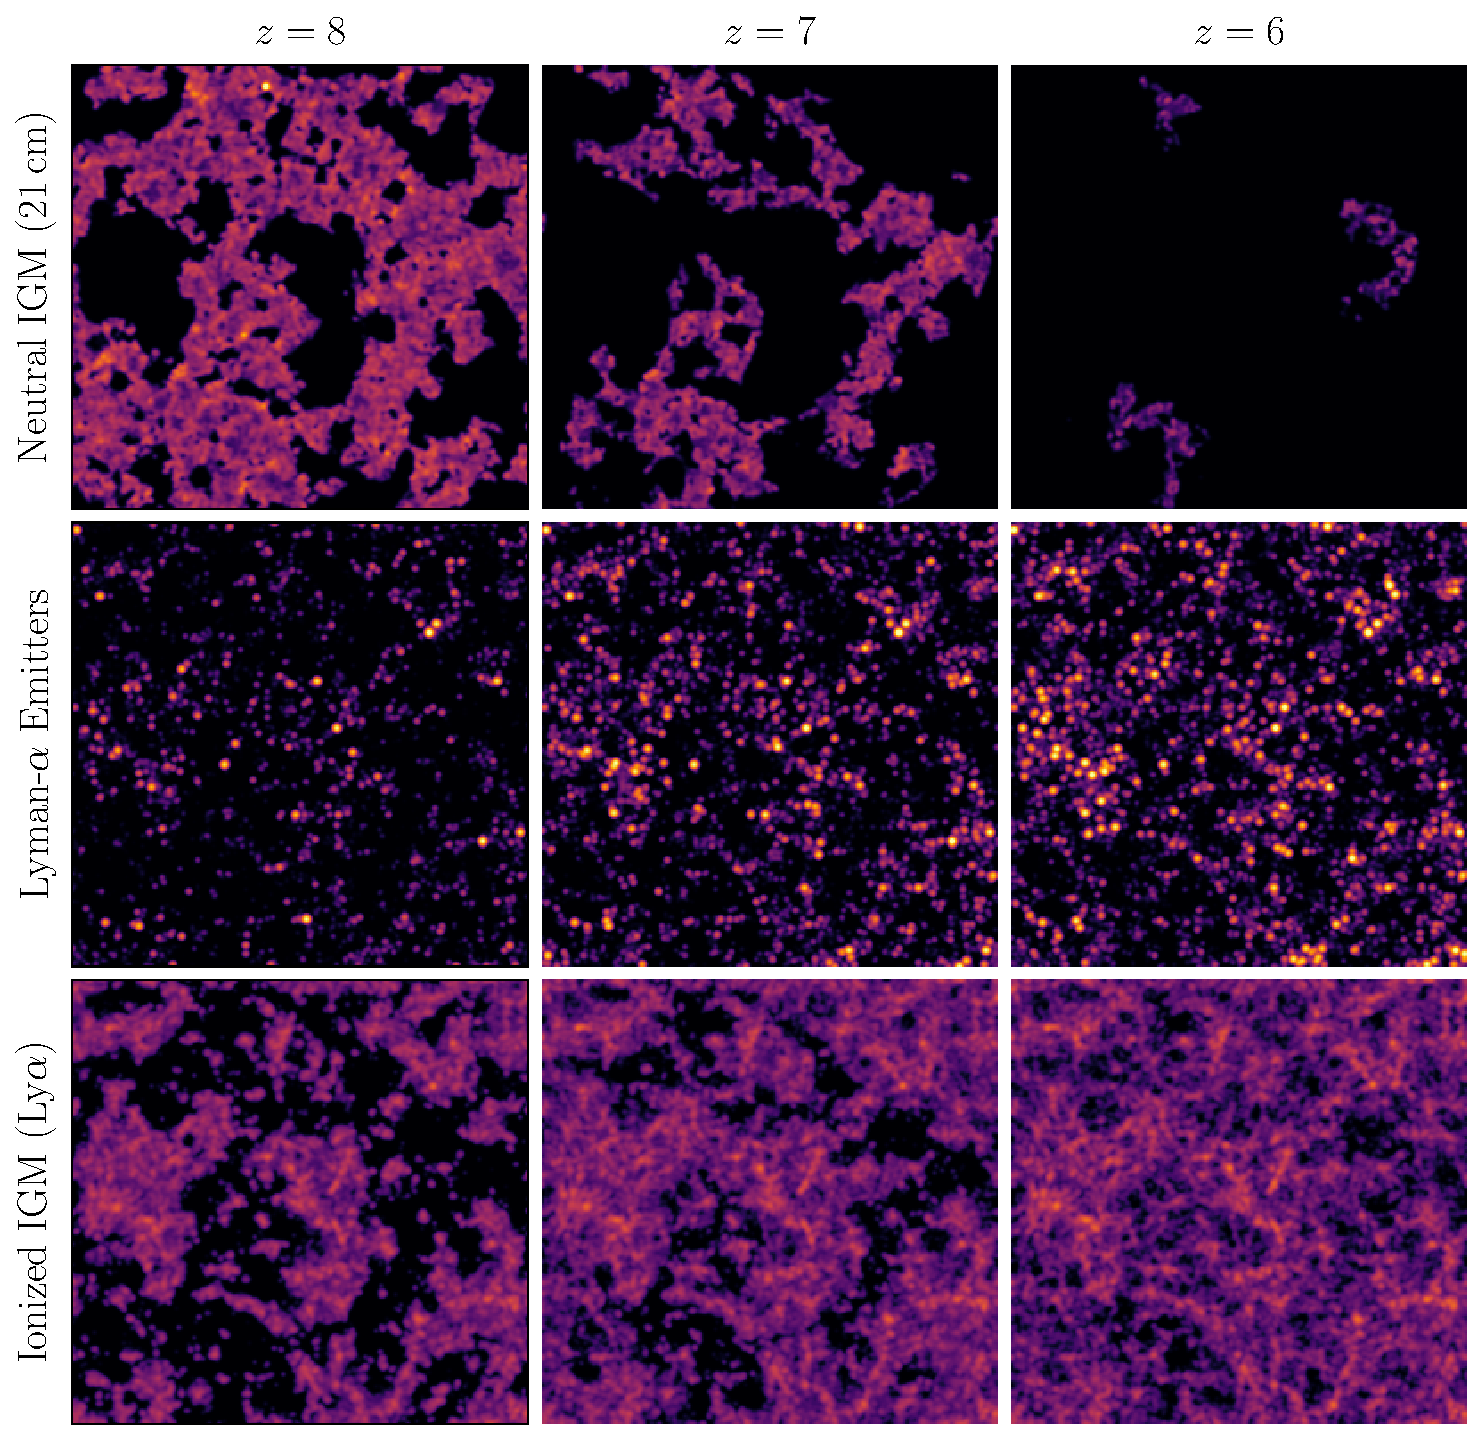
\includegraphics[width=1\textwidth]{sims.pdf}
	\caption[Simulated 21cm and \lya\ emission]{Slices through the simulated 21\,cm brightness temperature offset, $\delta T_b$, \lya\ emitter and ionized IGM cubes at $z = \left[6, 7, 8\right]$. Details on these simulations are described in Sections \hyperref[sec:21cm_temp]{2.1}, \hyperref[ref:laes]{2.2.1}, \hyperref[sec:ionized_igm]{2.2.2} respectively. The simulated box length is 200\,Mpc on a side. These fluctuation fields are used in later sections (Section \hyperref[sec:cross-power]{3.1}) to calculate the 21\,cm-\lya\ cross-power spectrum.}
	\label{fig:sims}
\end{figure}
